%%%%%%%%%%%%%%%%%%%%%%%%%%%%%%%%%%%%%%%%%%%%%%%%%%%%%%%%%%%%%%%%%%
%%%%%%%%% IEEEE Conference template enriched with stuffs %%%%%%%%%
%%%%%%%%%%%%%%%%%%%%%%%%%%%%%%%%%%%%%%%%%%%%%%%%%%%%%%%%%%%%%%%%%%
%%% The idea of this latex code is to support in the paper writing
%%% with helpful commands 
%%% (collected thanks to the many people that I collaborated with) and
%%% paper guidelines (e.g., https://www.youtube.com/watch?v=QYbAvOPcy0s)
%%%
%%% ACM conference/journal/sig* and IEEE transactions/journals 
%%% could reuse this structure/LaTeX commands easily
%%%%%%%%%%%%%%%%%%%%%%%%%%%%%%%%%%%%%%%%%%%%%%%%%%%%%%%%%%%%%%%%%%
%%%%%% by Davide Conficconi https://davideconficconi.github.io/ 
%%%%%%%%%%%%%%%%%%%%%%%%%%%%%%%%%%%%%%%%%%%%%%%%%%%%%%%%%%%%%%%%%%

\documentclass[conference]{IEEEtran}
\IEEEoverridecommandlockouts
% The preceding line is only needed to identify funding in the first footnote. If that is unneeded, please comment it out.
\usepackage{cite}
\usepackage{amsmath,amssymb,amsfonts}
\usepackage{algorithmic}
\usepackage{graphicx}
\usepackage{textcomp}
% \usepackage{xcolor} commented because reused afterwards
\def\BibTeX{{\rm B\kern-.05em{\sc i\kern-.025em b}\kern-.08em
    T\kern-.1667em\lower.7ex\hbox{E}\kern-.125emX}}

%%%package not from standard template
\usepackage[dvipsnames]{xcolor}
\usepackage{comment}
\usepackage{adjustbox}
\usepackage{listings}

\usepackage{booktabs} % For formal table
\usepackage{siunitx}
\usepackage{makecell}
\usepackage{multirow}
\usepackage{tabularx}
% \usepackage{subcaption}

\usepackage{lipsum}
\usepackage{algorithm}
\usepackage{tcolorbox}

%%% to balance references acrossy the columns
\usepackage{balance}

\usepackage{hyperref} 

%%% use color code plus comments to immediately show other authors
%%% the presence of additions or other things needs to be checked
\newcommand\myworries[1]{\textcolor{red}{#1}}
\newcommand\newtext[1]{\textcolor{blue}{#1}}
\newcommand{\orphan}[1]{\textcolor{magenta}{#1}}%magenta
\newcommand{\review}[1]{\textcolor{orange}{#1}}%orange
%%%this color is to define the whole table column with this color
\newcommand{\worrycolor}{\color{red}}

%%% to define a \blackcircled{whatsover} use this
\usepackage{tikz}
\newcommand*\blackcircled[1]{\tikz[baseline=(char.base)]{\node[shape=circle,fill,inner sep=0.7pt] (char) {\footnotesize{\textcolor{white}{#1}}};}}
\usepackage{pifont}
%%%%

%%% simple custom commands to use for sake of compactness
\newcommand{\gna}{\textsuperscript{$\dagger$}}
\newcommand{\gne}{\textsuperscript{$\ddagger$}}
\newcommand{\gno}{\textsuperscript{$\star$}}
\newcommand{\mytab}{\hspace{0.25cm}}

%%%if you have a tool/framework/something tha not know yet how to call it
%%use \tool across the manuscript for the sake of simplicity
\usepackage{xspace}
\newcommand{\tool}{\textsc{TritonBench}\xspace}


%%% define a better looking \CC{} latex
\def\CC{{C\nolinebreak[4]\hspace{-.05em}\raisebox{.4ex}{\tiny\bf ++}}\xspace}
%%%%%%%
\usepackage{cleveref}
\usepackage{url}
%if you are using cleveref this will show the sec ref with the \S symbol
\crefformat{section}{\S#2#1#3} % see manual of cleveref, section 8.2.1
\crefformat{subsection}{\S#2#1#3}
\crefformat{subsubsection}{\S#2#1#3}

\usepackage{circledsteps}
%this package let u use \Circled{whatever}
%

\definecolor{pairedOneLightBlue}{HTML}{a6cee3}
\definecolor{pairedTwoDarkBlue}{HTML}{1f78b4}
\definecolor{pairedThreeLightGreen}{HTML}{b2df8a}
\definecolor{pairedFourDarkGreen}{HTML}{33a02c}
\definecolor{pairedFiveLightRed}{HTML}{fb9a99}
\definecolor{pairedSixDarkRed}{HTML}{e31a1c}
\definecolor{butter1}{rgb}{0.988,0.914,0.310}
\definecolor{butter2}{rgb}{0.929,0.831,0.000}
\definecolor{butter3}{rgb}{0.769,0.627,0.000}
\definecolor{orange1}{rgb}{0.988,0.686,0.243}
\definecolor{orange2}{rgb}{0.961,0.475,0.000}
\definecolor{orange3}{rgb}{0.808,0.361,0.000}
\definecolor{chocolate1}{rgb}{0.914,0.725,0.431}
\definecolor{chocolate2}{rgb}{0.757,0.490,0.067}
\definecolor{chocolate3}{rgb}{0.561,0.349,0.008}
\definecolor{chameleon1}{rgb}{0.541,0.886,0.204}
\definecolor{chameleon2}{rgb}{0.451,0.824,0.086}
\definecolor{chameleon3}{rgb}{0.306,0.604,0.024}
\definecolor{skyblue1}{rgb}{0.447,0.624,0.812}
\definecolor{skyblue2}{rgb}{0.204,0.396,0.643}
\definecolor{skyblue3}{rgb}{0.125,0.290,0.529}
\definecolor{plum1}{rgb}{0.678,0.498,0.659}
\definecolor{plum2}{rgb}{0.459,0.314,0.482}
\definecolor{plum3}{rgb}{0.361,0.208,0.400}
\definecolor{scarletred1}{rgb}{0.937,0.161,0.161}
\definecolor{scarletred2}{rgb}{0.800,0.000,0.000}
\definecolor{scarletred3}{rgb}{0.643,0.000,0.000}
\definecolor{aluminium1}{rgb}{0.933,0.933,0.925}
\definecolor{aluminium2}{rgb}{0.827,0.843,0.812}
\definecolor{aluminium3}{rgb}{0.729,0.741,0.714}
\definecolor{aluminium4}{rgb}{0.533,0.541,0.522}
\definecolor{aluminium5}{rgb}{0.333,0.341,0.325}
\definecolor{aluminium6}{rgb}{0.180,0.204,0.212}

%% color scheme: 3 colors
\definecolor{blind_safe_one_scheme_three_colors}{RGB}{102,194,165}
\definecolor{blind_safe_two_scheme_three_colors}{RGB}{252,141,98}
\definecolor{blind_safe_three_scheme_three_colors}{RGB}{141,160,203}

%% color scheme: 4 colors
\definecolor{blind_safe_one_scheme_four_colors}{RGB}{166,206,227}
\definecolor{blind_safe_two_scheme_four_colors}{RGB}{31,120,180}
\definecolor{blind_safe_three_scheme_four_colors}{RGB}{178,223,138}
\definecolor{blind_safe_four_scheme_four_colors}{RGB}{51,160,44}

%% color scheme: 5 colors
\definecolor{blind_safe_one_scheme_five_colors}{RGB}{240,249,232}
\definecolor{blind_safe_two_scheme_five_colors}{RGB}{186,228,188}
\definecolor{blind_safe_three_scheme_five_colors}{RGB}{123,204,196}
\definecolor{blind_safe_four_scheme_five_colors}{RGB}{67,162,202}
\definecolor{blind_safe_five_scheme_five_colors}{RGB}{8,104,172}

%% color scheme: 7 colors
\definecolor{blind_safe_one_scheme_seven_colors}{RGB}{118,42,131}
\definecolor{blind_safe_two_scheme_seven_colors}{RGB}{175,141,195}
\definecolor{blind_safe_three_scheme_seven_colors}{RGB}{231,212,232}
\definecolor{blind_safe_four_scheme_seven_colors}{RGB}{247,247,247}
\definecolor{blind_safe_five_scheme_seven_colors}{RGB}{217,240,211}
\definecolor{blind_safe_six_scheme_seven_colors}{RGB}{127,191,123}
\definecolor{blind_safe_seven_scheme_seven_colors}{RGB}{27,120,55}

%% color scheme yellow-based 5 colors
\definecolor{yellow_one}{RGB}{255,255,212}
\definecolor{yellow_two}{RGB}{254,217,142}
\definecolor{yellow_three}{RGB}{254,153,41}
\definecolor{yellow_four}{RGB}{217,95,14}
\definecolor{yellow_five}{RGB}{153,52,4}

%% Colors for algo comments

\definecolor{forestgreen}{RGB}{34, 139, 34}

%% Colors of pipeline stages
\definecolor{pipeline_colors_fetch}{HTML}{80b1d3}
\definecolor{pipeline_colors_decode}{HTML}{e5c494}
\definecolor{pipeline_colors_rename}{HTML}{bebada}
\definecolor{pipeline_colors_dispatch}{HTML}{fb8072}
\definecolor{pipeline_colors_issue}{HTML}{d9d9d9}
\definecolor{pipeline_colors_execute}{HTML}{ffffb3}
\definecolor{pipeline_colors_commit}{HTML}{fccde5}


%
\usepackage{ifthen}
\usepackage{amssymb}

\newboolean{showcomments}
\setboolean{showcomments}{true}

% use \setboolean{showcomments}{false} anywhere in your document after
% importing this to disable the comments

\makeatletter
\newcommand{\mynote}[3]{%
  \ifthenelse{\boolean{showcomments}}{%
   \fbox{\bfseries\sffamily\scriptsize#1}%
   {\small$\blacktriangleright$\textsf{\emph{\color{#3}{#2}}}$\blacktriangleleft$}}%
  {%
   % these two lines ensure that there is no blank space inserted
   \@bsphack
   \@esphack
  }%
}
\makeatother

\newcommand{\rebuttal}[2]{\textcolor{#2}{#1}}

% One command per author:
\definecolor{asparagus}{rgb}{0.53, 0.66, 0.42}

\newcommand{\pone}[1]{\mynote{person1}{#1}{orange}}
\newcommand{\ptwo}[1]{\mynote{person2}{#1}{ForestGreen}}
\newcommand{\pthree}[1]{\mynote{person3}{#1}{Plum}}
\newcommand{\pfour}[1]{\mynote{person4}{#1}{BrickRed}}
%%%command to illustrate some good practice
%%% some are from https://www.youtube.com/watch?v=QYbAvOPcy0s
\newcommand{\goodpractice}[1]{\mynote{Goodpractice}{#1}{BrickRed}}
\newcommand{\prsop}[1]{\mynote{Personal Opinion}{#1}{Fuchsia}}
%
\usepackage[printonlyused]{acronym}
%
\acrodef{PL}[PL]{Programmable Logic}
\acrodef{PS}[PS]{Processing System}
\acrodef{HPE}[HPE]{Histogram PE}
\acrodef{EPE}[EPE]{Entropy PE}
\acrodef{AIE}[AIE]{AI Engine}
\acrodef{MI}[MI]{Mutual Information}
\acrodef{NoC}[NoC]{Network-on-Chip}
\acrodef{SM}[SM]{Similarity Metric}
\acrodef{FPGA}[FPGA]{Field Programmable Gate Array}
\acrodef{GPU}[GPU]{Graphical Processing Unit}
\acrodef{MSE}[MSE]{Mean Squared Error}
\acrodef{RMSE}[RMSE]{Root Mean Squared Error}
\acrodef{CC}[CC]{Cross Correlation}
\acrodef{SCC}[SCC]{Squared Cross Correlation}
\acrodef{PSNR}[PSNR]{Peak Signal-to-Noise Ratio}
\acrodef{NCC}[NCC]{Normalized Cross Correlation}
\acrodef{DSE}[DSE]{Design Space Exploration}
\acrodef{ASIC}[ASIC]{Application-Specific Integrated Circuit}
\acrodef{VLIW}[VLIW]{Very Long Instruction Word}
\acrodef{SLR}[SLR]{Super Logic Region}
\acrodef{HLS}[HLS]{High Level Synthesis}
\acrodef{HDL}[HDL]{Hardware Description Language}
\acrodef{NoC}[NoC]{Network on Chip}
\acrodef{SLR}[SLR]{Super Logic Region}
%

\begin{document}

\title{Triton vs. CUDA: A Workload-Driven Performance Analysis on Modern GPUs\\
{\footnotesize \textsuperscript{*}Focus on Structured vs. Irregular (FSM) Workloads}
}

\author{
\IEEEauthorblockN{Alessandro Potenza}
\IEEEauthorblockA{\textit{NECST Laboratory, DEIB} \\
\textit{Politecnico di Milano}\\
Milano, Italy \\
alessandro1.potenza@mail.polimi.it}
\and
\IEEEauthorblockN{Davide Conficconi}
\IEEEauthorblockA{\textit{NECST Laboratory, DEIB} \\
\textit{Politecnico di Milano}\\
Milano, Italy \\
davide.conficconi@mail.polimi.it}
\and
\IEEEauthorblockN{Filippo Del Nero}
\IEEEauthorblockA{\textit{NECST Laboratory, DEIB} \\
\textit{Politecnico di Milano}\\
Milano, Italy \\
filippo.delnero@mail.polimi.it}
}

\maketitle

\begin{abstract}
%
GPUs have become the engine of modern high-performance computing. While NVIDIA CUDA remains the industry standard, its complexity creates a high barrier to entry. OpenAI Triton, a Python-based DSL, aims to democratize GPU programming through a block-based model. While Triton excels at dense deep learning primitives, its capability to handle irregular, latency-bound workloads remains an open question.

This paper presents a workload-driven performance analysis comparing Triton and CUDA across two domains: structured, data-parallel computations (Matrix Multiplication) and irregular, control-flow intensive tasks (Finite State Machine simulation).
Our results show that for structured workloads, Triton achieves performance parity with CUDA. For irregular workloads involving pointer-chasing and divergent control flow, CUDA kernels are 10--30$\times$ faster than the best Triton implementations. We conclude that while Triton increases productivity for dense linear algebra, low-level CUDA remains essential for high-performance irregular algorithms.

%
\end{abstract}

\begin{IEEEkeywords}
GPGPU, CUDA, Triton, Finite State Machines, Irregular Workloads, Performance Analysis
\end{IEEEkeywords}

%
\section{Introduction}\label{sec:intro}

GPUs have become an indispensable driving force behind a wide range of applications. NVIDIA's CUDA \cite{cuda} has dominated this environment for over a decade, providing a programming model that exposes low-level hardware details. This results in maximum theoretical performance but presents a significant barrier to entry due to its complexity.

In response to this productivity challenge, higher-level abstractions have emerged. Among the most popular is Triton \cite{triton}, a Python-based DSL developed by OpenAI. Triton seeks to democratize GPU programming by allowing developers to write computations on data blocks, letting its JIT compiler handle memory coalescing and shared memory management.
While Triton has proven successful for dense neural network layers, this poses a challenging question: \textit{To what extent can a high-level block-based abstraction rival the performance of low-level CUDA across different computational problems?}

This paper addresses this question through a workload-driven comparative study. We benchmark two radically different types of workloads:
\begin{itemize}
    \item \textbf{Structured Workloads:} Problems like Matrix Multiplication, characterized by uniform data access and deterministic control flow.
    \item \textbf{Irregular Workloads:} Problems like Finite State Machine (FSM) simulation, characterized by sparse memory accesses (pointer-chasing) and divergent control flow.
\end{itemize}

The main contributions of this paper are:
\begin{enumerate}
    \item A performance comparison of Triton and CUDA kernels on both structured (MatMul) and irregular (FSM) computational domains.
    \item An implementation of specialized FSM kernels in Triton (Bitmap, CSR, DFS) compared against CUDA approaches.
    \item An analysis of the performance gap observed in irregular workloads, relating them to the programming model design.
\end{enumerate}

Our principal thesis is that the optimal programming model is workload-dependent. While Triton achieves performance parity for structured computations, the low-level control offered by CUDA is essential for irregular workloads. We show that for FSM simulation, CUDA kernels outperform Triton by 10--30$\times$ due to the latter's inability to efficiently handle fine-grained latency-bound operations.

%
\section{Background}\label{sec:background}

To understand the performance analysis presented in this work, it is essential to first grasp the fundamental differences between the programming models under investigation and the characteristics of the workloads used for evaluation.

\subsection{GPU Programming Models}

\subsubsection{CUDA C++ (The Baseline)}
NVIDIA's CUDA \cite{cuda} adopts a Single Instruction Multiple Thread (SIMT) execution model. It grants developers direct and explicit control over the GPU architecture. Programmers manage the thread hierarchy (grid, blocks, and warps), handle memory transfers between host and device, and manually optimize memory access patterns to maximize bandwidth (e.g., ensuring coalesced global memory reads).
This fine-grained control allows for sophisticated optimizations, such as using \textit{Warp Shuffle} primitives for register-level communication or managing Shared Memory to reduce global traffic. However, this comes at the cost of high code verbosity and complexity.

\subsubsection{OpenAI Triton (The Abstraction)}
Triton \cite{triton} introduces a block-based programming model. Instead of writing code for a single thread (as in CUDA), the developer writes operations on blocks of data (tensors). The Triton compiler automatically handles the complex tasks of multi-threading, shared memory allocation, and synchronization barriers.
While this abstraction simplifies the development of dense matrix operations, it hides the concept of an individual thread ID. This makes it difficult to express algorithms that require per-thread logic or random access patterns, as operations must be defined over entire blocks.

\subsection{Workload Characterization}

The success of a GPU programming model relies significantly on the nature of the target workload. We classify our benchmarks into two broad categories:

\subsubsection{Structured Workloads}
These applications represent the classical use case for GPUs, such as Dense Neural Network layers and Matrix Multiplication. They are characterized by:
\begin{itemize}
    \item \textbf{Predictable Memory Access:} Threads read memory in contiguous sequences, enabling fully coalesced loads.
    \item \textbf{High Arithmetic Intensity:} A high ratio of compute operations to memory references.
    \item \textbf{Uniform Control Flow:} All threads in a warp typically follow the same execution path.
\end{itemize}
These characteristics map perfectly to Triton's block-level semantics.

\subsubsection{Irregular Workloads}
This class of problems exposes the limits of parallel architectures. We utilize Finite State Machine (FSM) simulation as our representative irregular workload. FSM processing is characterized by:
\begin{itemize}
    \item \textbf{Pointer Chasing:} To evaluate the next state, the algorithm must read a value from a memory location determined by the current state ($S_{t+1} = \delta(S_t, Input)$). This results in scattered, non-coalesced memory accesses.
    \item \textbf{Sequential Dependency:} The next state depends entirely on the previous one, creating a strict latency-bound chain that is hard to pipeline.
    \item \textbf{Divergent Control Flow:} Different input strings may lead to different states, causing threads in a warp to diverge and serialize execution.
\end{itemize}
%
\section{Methodology}\label{sec:method}

This section details the experimental setup, the system configuration, and the specific algorithms implemented to compare the programming models.

\subsection{System Configuration}
All benchmarks were executed on a consistent hardware platform to ensure fair comparisons.
\begin{itemize}
    \item \textbf{GPU:} NVIDIA GeForce RTX 4070 (Ada Lovelace, 12GB GDDR6X).
    \item \textbf{Software Stack:} CUDA Toolkit 12.3, PyTorch 2.1, Triton 2.1.
    \item \textbf{Environment:} A strictly controlled Docker container to ensure reproducibility of the Python/C++ build environment.
\end{itemize}

\subsection{Algorithm Implementation Details}

Our core investigation focuses on the contrast between high-level and low-level implementations of FSM simulation.

\subsubsection{Triton Implementation (High-Level)}
The Triton kernel adopts a ``dense'' approach to fit the block-based programming model. It tracks active states using a boolean tensor or sparse list, but relies on masked loads to handle the irregularity of the transition table.
As shown in Algorithm \ref{alg:triton}, the absence of per-thread branching forces the compiler to emit predicated instructions that execute both the memory load and the validity check, often reading unnecessary data (over-fetching).

\begin{algorithm}[h]
\caption{Triton CSR Kernel Logic (Simplified)}
\label{alg:triton}
\begin{algorithmic}[1]
\STATE \textbf{Input:} $state\_id, input\_char$
\STATE $row\_start \leftarrow \textbf{tl.load}(row\_ptr + state\_id)$
\STATE $row\_end \leftarrow \textbf{tl.load}(row\_ptr + state\_id + 1)$
\STATE $curr \leftarrow row\_start$
\WHILE{$curr < row\_end$}
    \STATE \textit{// Masked Load required for irregular access}
    \STATE $sym \leftarrow \textbf{tl.load}(data + curr, \textbf{mask}=curr < row\_end)$
    \STATE $target \leftarrow \textbf{tl.load}(indices + curr, \textbf{mask}=curr < row\_end)$
    \IF{$sym == input\_char$}
        \STATE \textbf{tl.atomic\_store}(next\_state, target)
    \ENDIF
    \STATE $curr \leftarrow curr + 1$
\ENDWHILE
\end{algorithmic}
\end{algorithm}

\subsubsection{CUDA Implementation (Low-Level)}
The CUDA kernel implements the \textit{ngAP} (N-Grams Automata Processor) strategy \cite{ngap}. It utilizes a global worklist to balance load and specialized hardware intrinsics.
As shown in Algorithm \ref{alg:cuda}, we explicitly manage the cache hierarchy using the `\_\_ldg` intrinsic (read-only cache) and reduce global memory contention by aggregating atomic updates at the warp level using `\_\_ballot\_sync`.

\begin{algorithm}[h]
\caption{CUDA ngAP Kernel Logic (Optimized)}
\label{alg:cuda}
\begin{algorithmic}[1]
\STATE \textbf{Input:} $worklist$ (Shared Memory / Global)
\STATE $state\_id \leftarrow \text{pop\_work\_item}(worklist)$
\STATE \textit{// Read-Only Cache Optimization}
\STATE $row\_start \leftarrow \textbf{\_\_ldg}(row\_ptr + state\_id)$
\STATE \FOR{$i \leftarrow row\_start$ \textbf{to} $row\_end$}
    \STATE $sym \leftarrow \textbf{\_\_ldg}(data + i)$
    \IF{$sym == input\_char$}
        \STATE $next \leftarrow \textbf{\_\_ldg}(indices + i)$
        \STATE \textit{// Warp Aggregation to reduce global atomics}
        \STATE $vote \leftarrow \textbf{\_\_ballot\_sync}(FULL\_MASK, true)$
        \IF{lane\_id == \textbf{\_\_ffs}(vote) - 1}
            \STATE \textbf{atomicAdd}(global\_queue, popc(vote))
        \ENDIF
    \ENDIF
\ENDFOR
\end{algorithmic}
\end{algorithm}

\subsection{Benchmark Metrics}
We evaluate performance using the following metrics:
\begin{itemize}
    \item \textbf{Kernel Execution Time (ms):} The raw time spent by the GPU to execute the compute kernel.
    \item \textbf{System Overhead:} The time spent in driver latency, JIT compilation, and data movement, calculated as $T_{Total} - T_{Kernel}$.
    \item \textbf{Speedup:} Defined as $T_{Triton} / T_{CUDA}$.
\end{itemize}
%
\section{Results and Analysis}\label{sec:results}

This section presents our experimental results across four dimensions: structured workload parity, the irregular workload performance gap, CUDA technique comparison, and the productivity-performance trade-off.

\subsection{Structured Workloads: Parity}

For structured, data-parallel workloads, Triton delivers on its promise. Fig.~\ref{fig:structured} shows results for Matrix Multiplication and Multi-Layer Perceptron (MLP) forward passes.

\textbf{Matrix Multiplication.} Triton achieves near-parity with cuBLAS across matrix sizes. At $1024^3$, Triton is $1.08\times$ slower (0.156~ms vs 0.145~ms). At $2048^3$, Triton matches cuBLAS ($0.99\times$, 0.959~ms vs 0.967~ms). At $4096^3$, the gap widens to $1.27\times$ (8.06~ms vs 6.35~ms), likely due to cache optimization in cuBLAS.

\textbf{MLP Forward Pass.} For MLP workloads, Triton achieves parity or better ($0.75\times$--$1.20\times$). The best Triton implementations leverage kernel fusion, avoiding intermediate memory writes between layers. For example, at configuration $512{\times}2048{\times}4096{\times}1024$, fused Triton achieves 0.58~ms compared to 0.77~ms for cuBLAS-based CUDA.

These results confirm that Triton's block-based abstraction maps well to hardware tensor cores for dense algebra with negligible abstraction cost.

\begin{figure}[htbp]
    \centering
    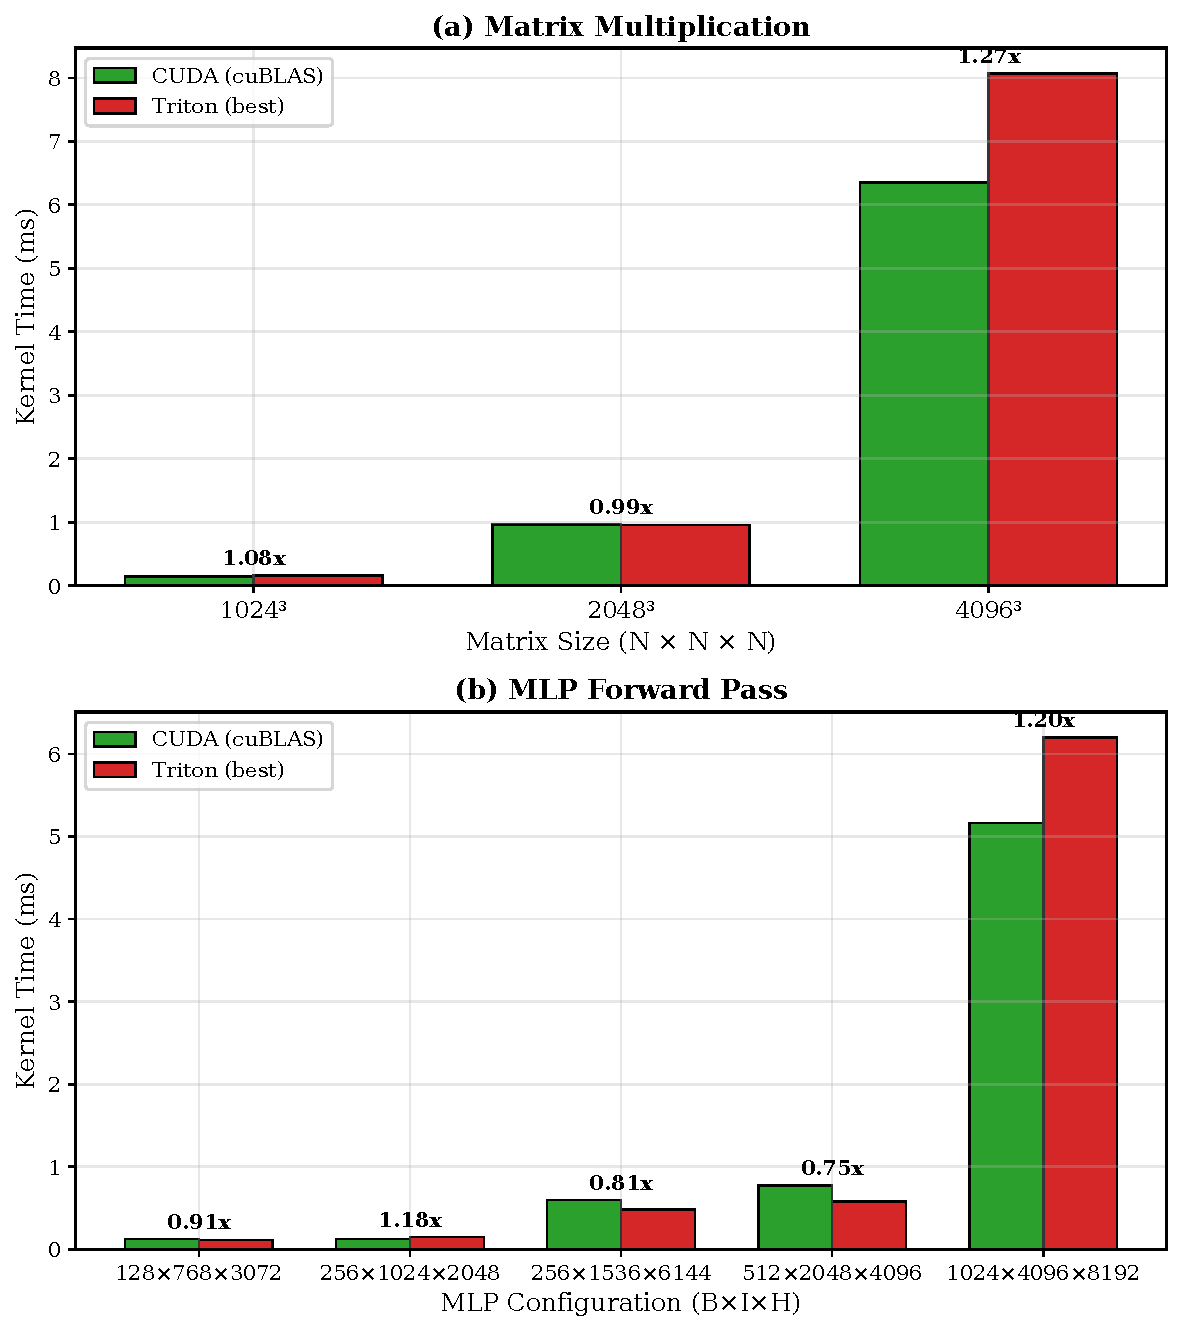
\includegraphics[width=\linewidth]{figures/fig_structured_parity.pdf}
    \caption{Structured Workloads. (a) Matrix Multiplication: Triton achieves $0.99\times$--$1.27\times$ vs cuBLAS. (b) MLP Forward Pass: Triton achieves $0.75\times$--$1.20\times$, with kernel fusion providing speedups on larger models.}
    \label{fig:structured}
\end{figure}

\subsection{Irregular Workloads: The Gap}

The scenario changes for Finite State Machines (FSM). Fig.~\ref{fig:fsm_gap} shows the performance gap on a logarithmic scale.

CUDA implementations outperform Triton by 10--30$\times$ (median: 10$\times$). This gap is structural:
\begin{itemize}
    \item \textbf{Latency-Bound:} FSM processing requires reading single bytes at random locations. Triton's \texttt{tl.load} fetches blocks, causing bus under-utilization.
    \item \textbf{Control Flow:} Triton handles conditionals via masking. CUDA skips unnecessary work with thread-local logic.
\end{itemize}

\begin{figure}[htbp]
    \centering
    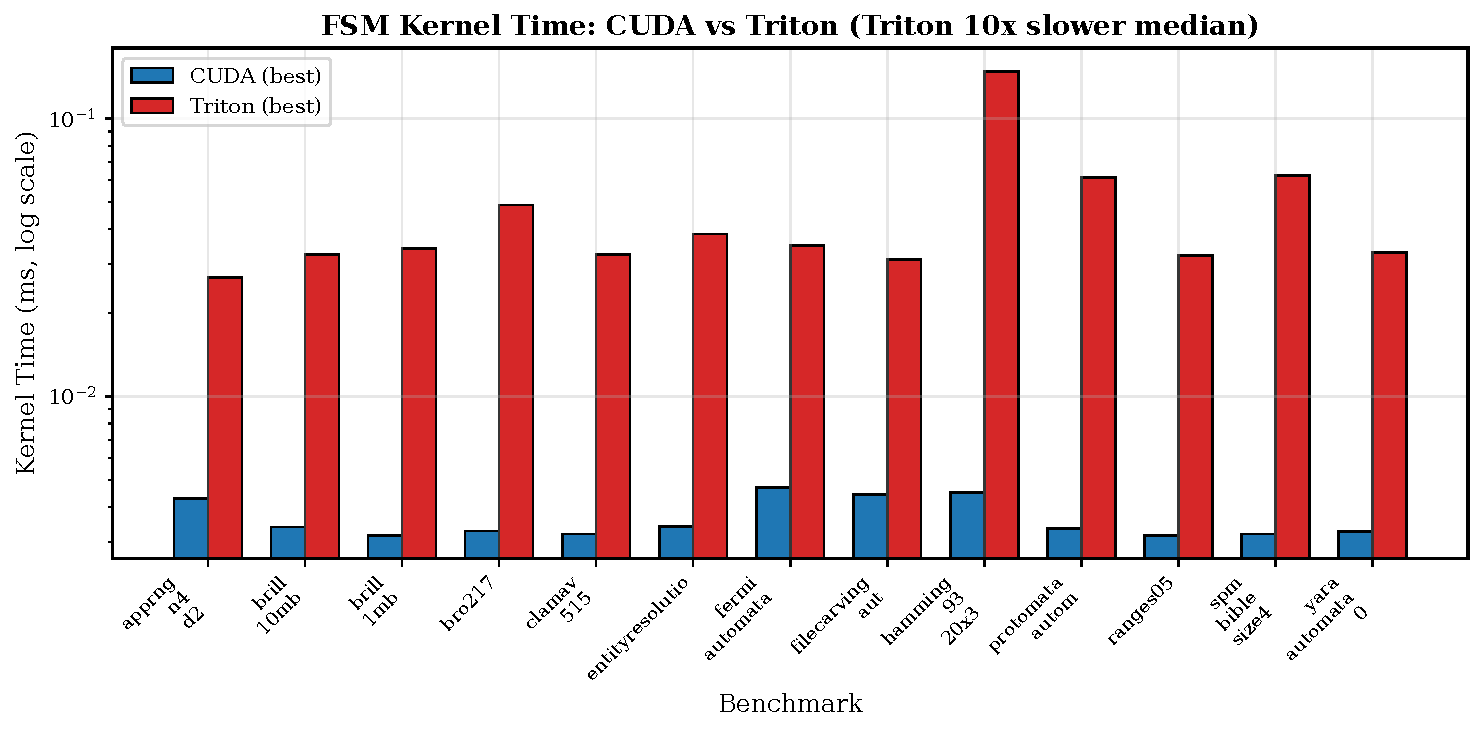
\includegraphics[width=\linewidth]{figures/fig_fsm_gap.pdf}
    \caption{The Irregularity Gap. CUDA kernels are 10--30$\times$ faster than Triton for FSM processing.}
    \label{fig:fsm_gap}
\end{figure}

\subsection{Technique Comparison: CUDA vs Triton}

Fig.~\ref{fig:cuda_techniques} compares FSM techniques from both CUDA and Triton across all benchmarks. CUDA techniques include Basic, CSR, ngAP, and BitGen. Triton techniques include DFS (best), CSR, and Bitmap.

\begin{figure*}[htbp]
    \centering
    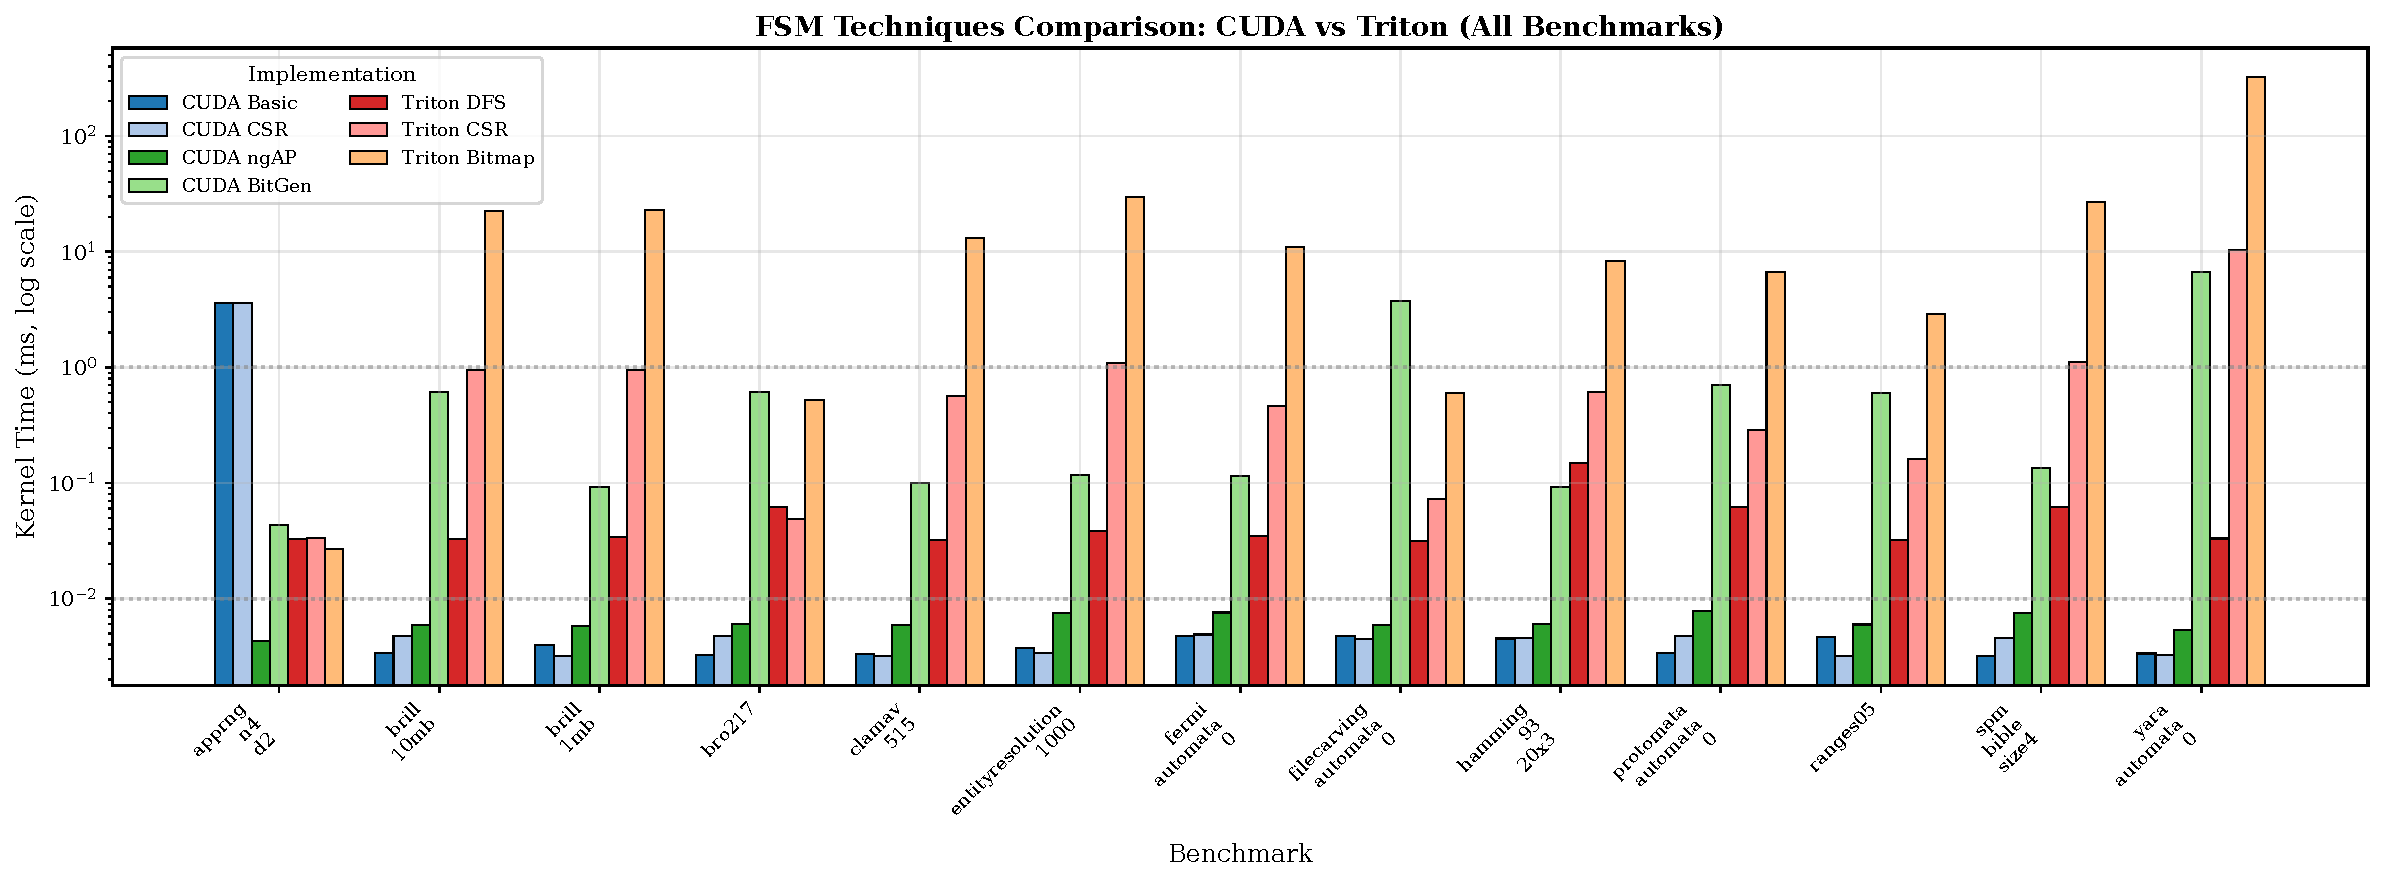
\includegraphics[width=\textwidth]{figures/fig_cuda_techniques.pdf}
    \caption{FSM Techniques Comparison: CUDA vs Triton. Blue/green bars show CUDA techniques (3--140~$\mu$s). Red/orange bars show Triton techniques (34~$\mu$s--15~ms). The gap is consistent across all benchmarks.}
    \label{fig:cuda_techniques}
\end{figure*}

Key findings:
\begin{itemize}
    \item \textbf{CUDA Basic/CSR:} Fastest overall (3--6~$\mu$s median). Simple serial traversal is effective when memory layout is optimized.
    \item \textbf{CUDA ngAP:} Comparable to Basic/CSR on single-stream workloads. ngAP~\cite{ngap} is designed for \emph{multi-stream} processing where thousands of input streams are processed in parallel. In our single-stream benchmark, the worklist overhead is not amortized.
    \item \textbf{CUDA BitGen:} Median 0.14~ms, slower than Basic for small inputs. BitGen~\cite{bitgen} transforms memory-bound workloads into compute-bound via bit-parallel operations. This approach benefits large-scale multi-pattern matching scenarios rather than single-stream processing.
    \item \textbf{Triton DFS:} Best Triton technique (34~$\mu$s median), but still $10\times$ slower than CUDA Basic.
    \item \textbf{Triton Bitmap:} Slowest approach (11--15~ms), $1000\times$ slower than CUDA Basic.
\end{itemize}

\textbf{Note on Advanced Techniques.} Both ngAP and BitGen are optimized for production scenarios with parallel input streams (e.g., network packet inspection processing thousands of packets simultaneously). Our single-stream benchmark favors simpler techniques. Production deployments should consider multi-stream batching where these advanced techniques may outperform Basic/CSR.

The gap between CUDA and Triton is consistent across all benchmarks and techniques, confirming the structural nature of the performance difference.

\subsection{Speedup Analysis}

Fig.~\ref{fig:speedup} shows the CUDA speedup over Triton for each FSM benchmark, sorted by magnitude. The speedup ranges from $6.2\times$ to $32.8\times$, with a median of $10.2\times$.

The benchmarks with highest speedup (brill, protomata, yara) involve complex automata with many states and transitions. The benchmarks with lower speedup (apprng, filecarving) have simpler structures where Triton's overhead is less pronounced.

\begin{figure}[htbp]
    \centering
    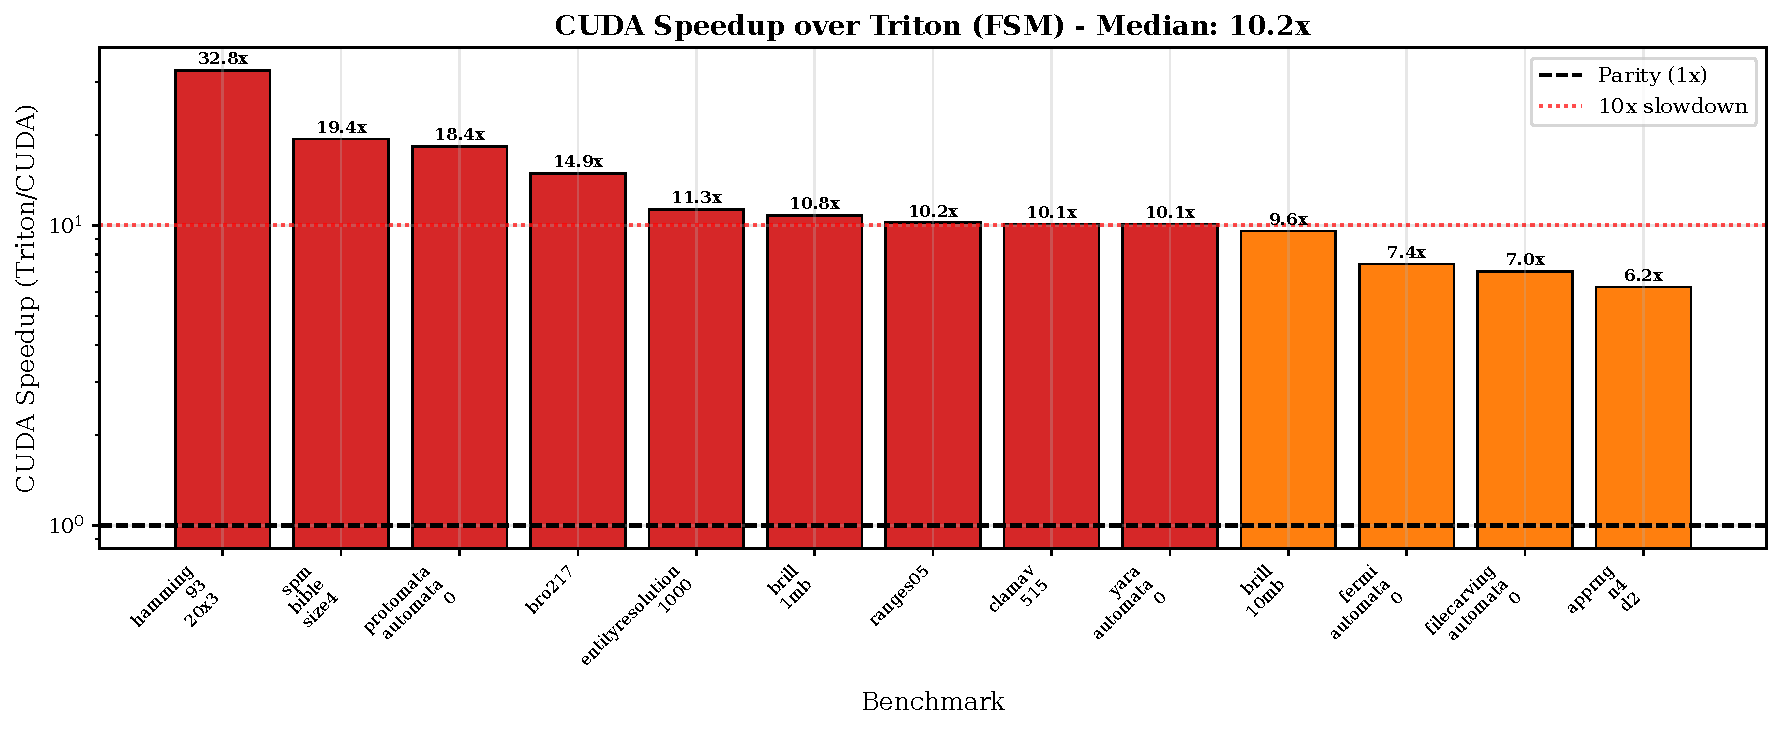
\includegraphics[width=\linewidth]{figures/fig_speedup_analysis.pdf}
    \caption{CUDA Speedup over Triton (FSM). Benchmarks sorted by speedup magnitude. Red bars indicate $>10\times$ slowdown, orange $5$--$10\times$, green $<5\times$.}
    \label{fig:speedup}
\end{figure}

\subsection{Productivity vs Performance Trade-off}

Fig.~\ref{fig:tradeoff} plots development effort (Lines of Code) against performance.

\begin{figure}[htbp]
    \centering
    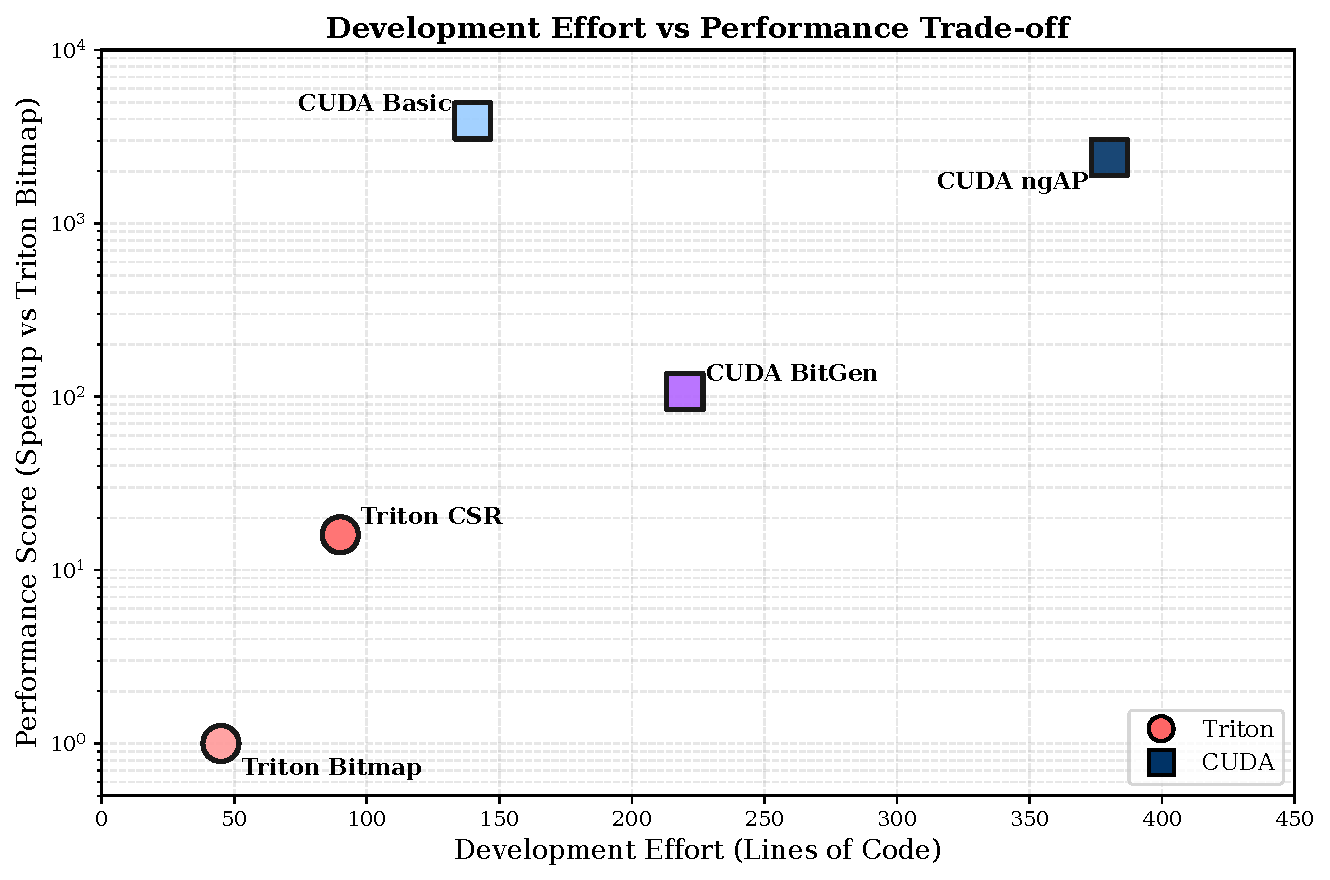
\includegraphics[width=\linewidth]{figures/fig_tradeoff.pdf}
    \caption{Productivity vs Performance. Triton allows concise code but hits a performance ceiling. CUDA techniques span a range of complexity and performance.}
    \label{fig:tradeoff}
\end{figure}

\begin{itemize}
    \item \textbf{Triton:} 45--60 LoC, lowest performance for FSM.
    \item \textbf{CUDA Basic/CSR:} 120--180 LoC, best performance for single-stream processing.
    \item \textbf{CUDA BitGen:} $\approx$250 LoC, competitive for multi-pattern workloads.
    \item \textbf{CUDA ngAP:} $\approx$380 LoC, complex implementation without proportional gains on our benchmark suite.
\end{itemize}

This demonstrates that for irregular workloads, the abstraction that makes Triton productive prevents expressing necessary low-level optimizations.

\subsection{System Overhead Analysis}

Fig.~\ref{fig:overhead} shows the breakdown between kernel execution time and system overhead (PCIe transfer, driver latency) for FSM workloads.

\begin{figure}[htbp]
    \centering
    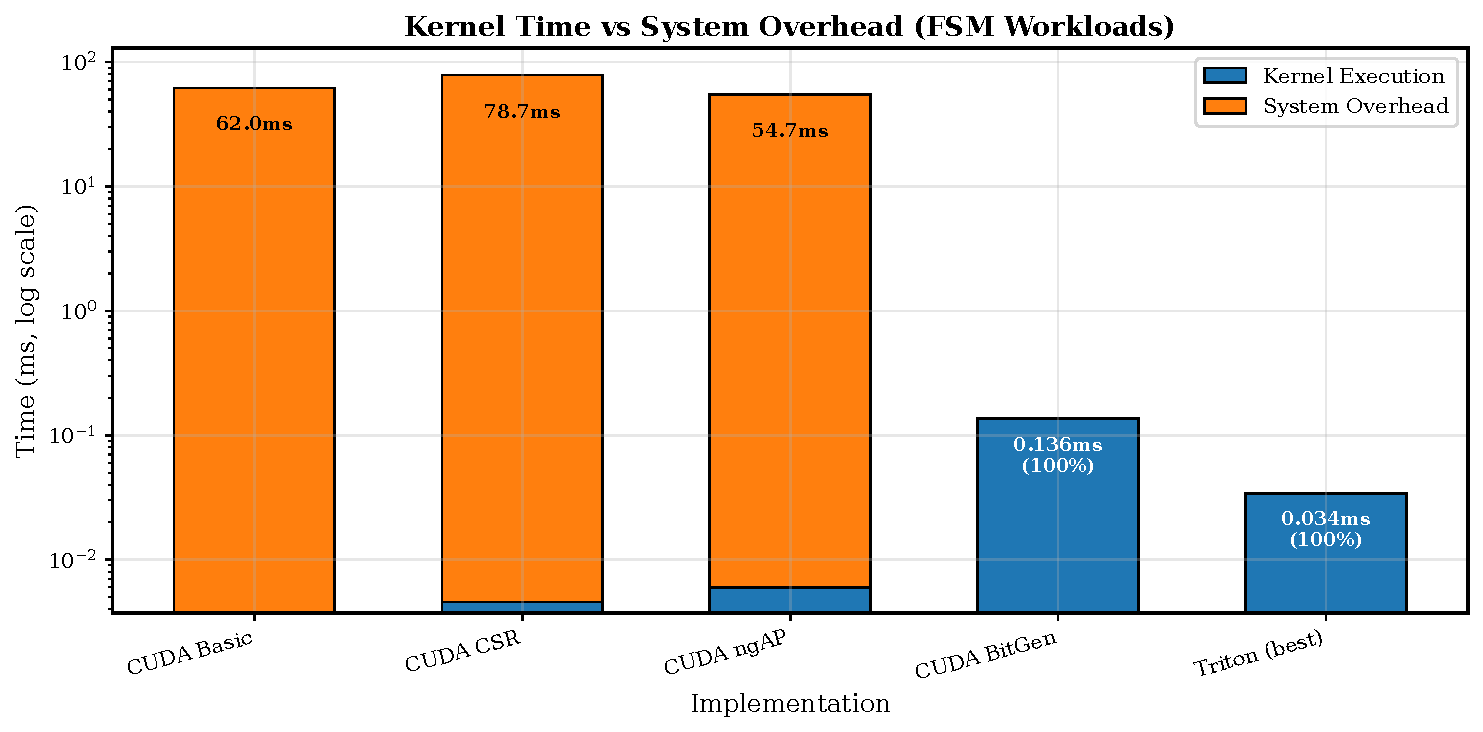
\includegraphics[width=\linewidth]{figures/fig_overhead.pdf}
    \caption{Kernel Time vs System Overhead. CUDA kernels are so fast (3--6~$\mu$s) that system overhead dominates total execution time.}
    \label{fig:overhead}
\end{figure}

For CUDA Basic/CSR, kernel execution represents less than 0.01\% of total time. The remaining 99.99\% is system overhead. This has important implications:
\begin{itemize}
    \item \textbf{Batching:} For production workloads, batching multiple FSM operations per kernel launch amortizes overhead.
    \item \textbf{Streaming:} Overlapping data transfer with computation can hide PCIe latency.
    \item \textbf{Triton advantage:} Triton's higher kernel time means overhead is proportionally smaller, making raw kernel comparisons misleading for end-to-end latency.
\end{itemize}

%
\section{Related Work}\label{sec:soa}

Our research bridges two bodies of literature: high-level GPU programming models and algorithmic optimization of automata processing.

\subsection{High-Level GPU Abstractions}

The complexity of CUDA has driven research into Domain-Specific Languages (DSLs).
\textbf{Triton}~\cite{triton} simplifies writing high-performance neural network kernels through a tile-based semantics where the compiler manages memory coalescing and shared memory allocation.
While Tillet et al.\ demonstrated Triton's effectiveness for matrix multiplications, their analysis was confined to dense linear algebra. Our work extends this evaluation to irregular, latency-bound algorithms.

\subsection{Parallel FSM Processing on GPUs}

Mapping Finite State Machines to GPUs is difficult due to sequential data dependencies.

\subsubsection{Speculative Approaches}
Mytkowicz et al.~\cite{mytkowicz2014} proposed enumeration-based parallelism, speculatively executing the FSM for all possible starting states. While effective on CPUs with SIMD, this approach has high overhead for single-stream processing.

\subsubsection{Memory-Centric Approaches}
Yaneva et al.~\cite{yaneva2017} analyzed memory layouts for FSM traversal, contrasting CSR against dense Transition Matrices. Our Triton implementation builds on these findings with both Bitmap and CSR variants.

\subsubsection{Worklist-Based Approaches}
Ge et al.\ proposed \textbf{ngAP}~\cite{ngap}, a non-blocking queue-based architecture using warp-level primitives for load balancing. We include ngAP-inspired implementations as a baseline, showing that the required hardware primitives (\texttt{warp\_shuffle}, fine-grained shared memory) are inexpressible in Triton.

\subsubsection{Bit-Parallel Approaches}
Recent work has explored bit-parallel methods that transform regex into bitstream programs.
\textbf{HybridSA}~\cite{hybridsa} (OOPSLA 2024) demonstrated CPU-GPU parallel engines using bit parallelism for NFA simulation, reducing irregular memory accesses.
\textbf{BitGen}~\cite{bitgen} (MICRO 2025) introduced interleaved bitstream execution, keeping intermediate data in registers rather than global memory. BitGen reports 19.5$\times$ speedup over ngAP by transforming the workload from memory-bound to compute-bound.
We evaluate BitGen in our benchmark suite to understand how bit-parallel approaches compare to traditional graph-traversal methods across different automata structures.

%
\section{Conclusion}\label{sec:conclusion}

In this paper, we presented a workload-driven performance analysis comparing OpenAI Triton and NVIDIA CUDA. We sought to determine if a modern block-based DSL could replace low-level code across diverse computational domains.

Our study leads to a nuanced conclusion: the optimal programming model depends on workload regularity.
\begin{itemize}
    \item \textbf{Structured Workloads:} Triton achieves performance parity with cuBLAS and offers significant productivity advantages. For dense algebra, the abstraction cost is effectively zero.
    \item \textbf{Irregular Workloads:} The abstraction breaks down. Block-based semantics introduce significant overhead for latency-bound, pointer-chasing algorithms. CUDA kernels outperform Triton by 10--30$\times$.
\end{itemize}

We identify this as \textit{Abstraction Regret}: the features that make Triton productive (block abstraction) prevent the expression of micro-optimizations required for irregular domains.
Future work should explore extending Triton's IR to support scalar intrinsics and worklist semantics, potentially bridging this gap.

%
\section*{Acknowledgment}
This work was supported by the NECST Laboratory at Politecnico di Milano. We thank the reviewers for their insightful feedback on the architectural analysis of the abstraction gap.
%
\balance
\def\UrlBreaks{\do\/\do-}
\bibliographystyle{IEEEtran}
\bibliography{bibliography}

\end{document}